\likechapter{ВВЕДЕНИЕ}
В нынешнее время технологии достигли уровня, когда автоматизированные системы используются повсеместно и тем не менее остаются не занятые ниши. На отечественном рынке медицинского оборудования очень малленький выбор устройств, которые могут измерить глубину аккомодации глаза (аккомодометров), а то небольшое количество видов устройств что есть(cм. рис.\ref{fig:aka-01}) не имеют электроприводов из-за чего движение внутренних механизмов осуществляется за счет мускульного усилия пациента, либо врача, так же на таких устройствах крайне не удобно выполнять тренировочные упражнения, которые достаточно важны для увеличения, либо для профилактики уменьшения глубины аккомодации.

Множество других недостатков по сравнению с автоматизированным устройством, где все измерения, запись параметров, создание журнала измерений, математики просчета средних и их погрешностей, формы конспекта осмотра врача для печати и много другое делается быстрее, с приложением наименьших усилий врача и пациента. С использование электроники можно создать новый, востребованное устройство, в этой работе поставлена задача создание автоматизированной системы современного аккомодометра(далее аппарата).
\begin{figure}[ht]
    \centering
    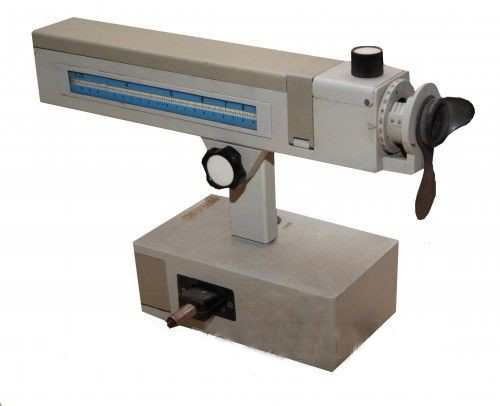
\includegraphics[scale=0.5]{akkomodometr-aka-01.jpg}
    \caption{Аккомодометр АКА-01.}
    \label{fig:aka-01}
\end{figure}	